

\chapter{预等离子体对于加速的增强作用}
\label{chap:preplasmaEhancement}

\section{预脉冲与预等离子体}
\begin{figure}[!htbp]
  \centering
  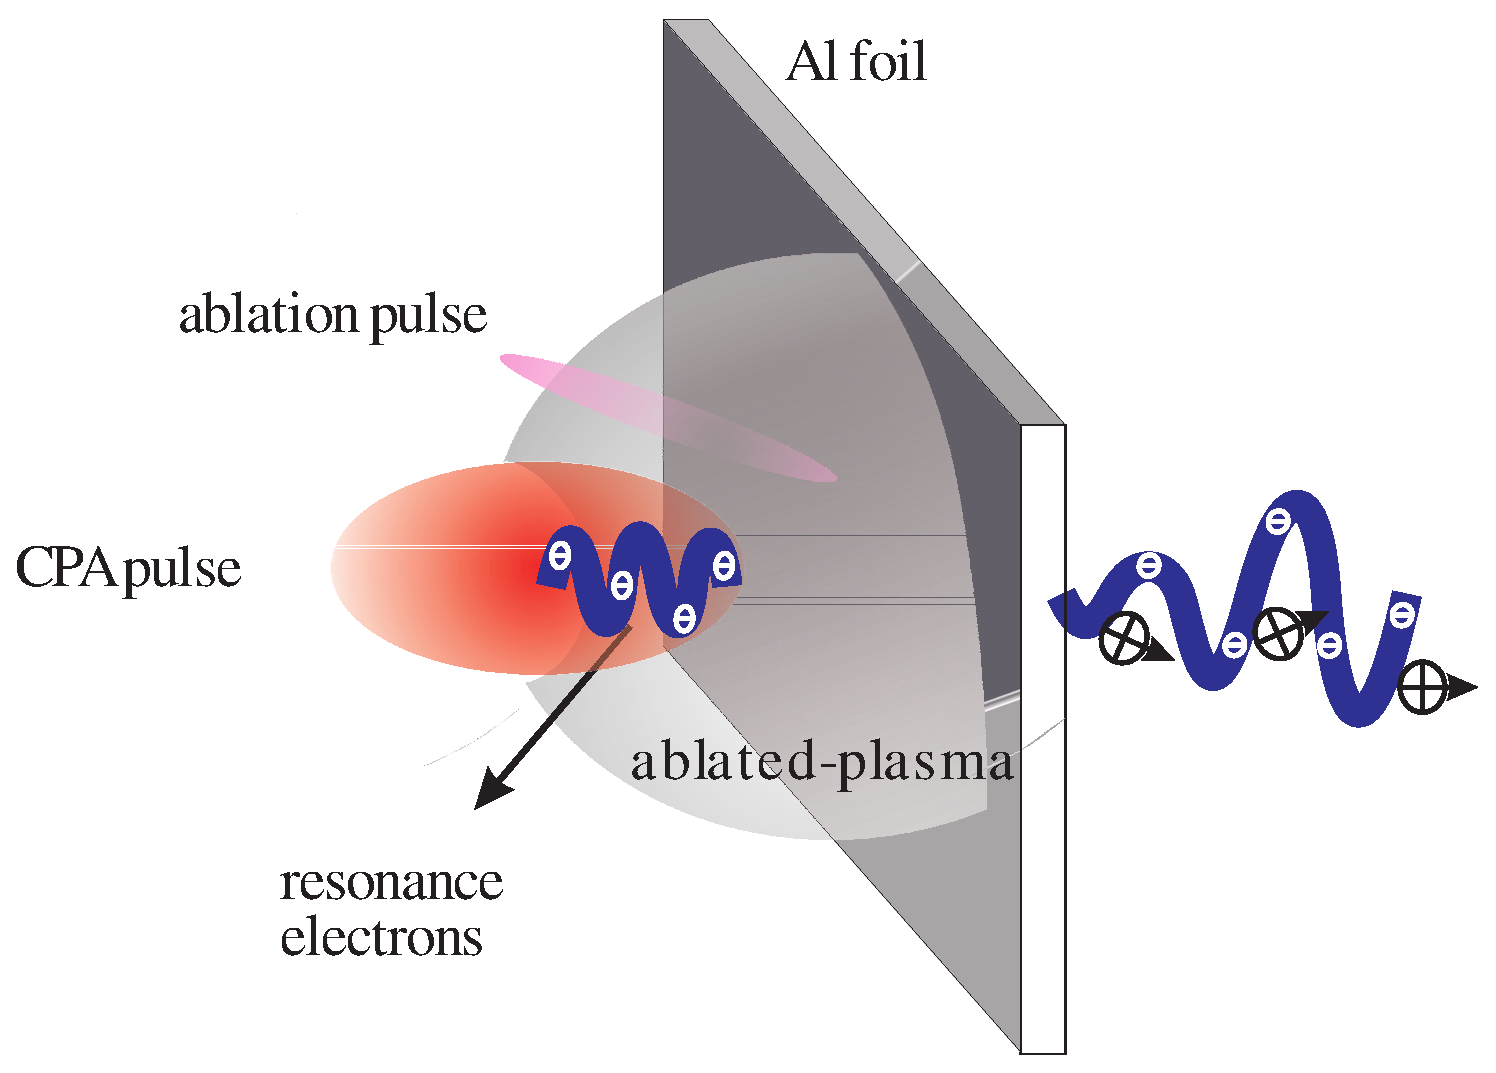
\includegraphics[width=\MyFactor\textwidth]{Img/enhancement.eps}
  \caption{预脉冲增强作用示意图}
  \label{fig:prepulse2012}
\end{figure}



上一章中,我们利用激光的预脉冲或者中等强度激光脉冲($10^{10}W/cm^2$ 到 $10^{14}W/cm^2$),对于金属靶进行烧蚀,产生预等离子体。预等离子体由靶前表面向外传播,其密度一维分布为类指数函数,其中一部分处于临界密度领域。我们已经对于临界密度做出定义,与激光频率一致的等离子体波对应的密度,同时也是非相对论激光脉冲穿透密度极限。而当激光的光强到达相对论区域,等离子体频率由于相对论效应相应地降低,因此激光穿透等离子体的能力增强,而此时等离子体也称为临界密度等离子体。

\begin{figure}[!htbp]
  \centering
  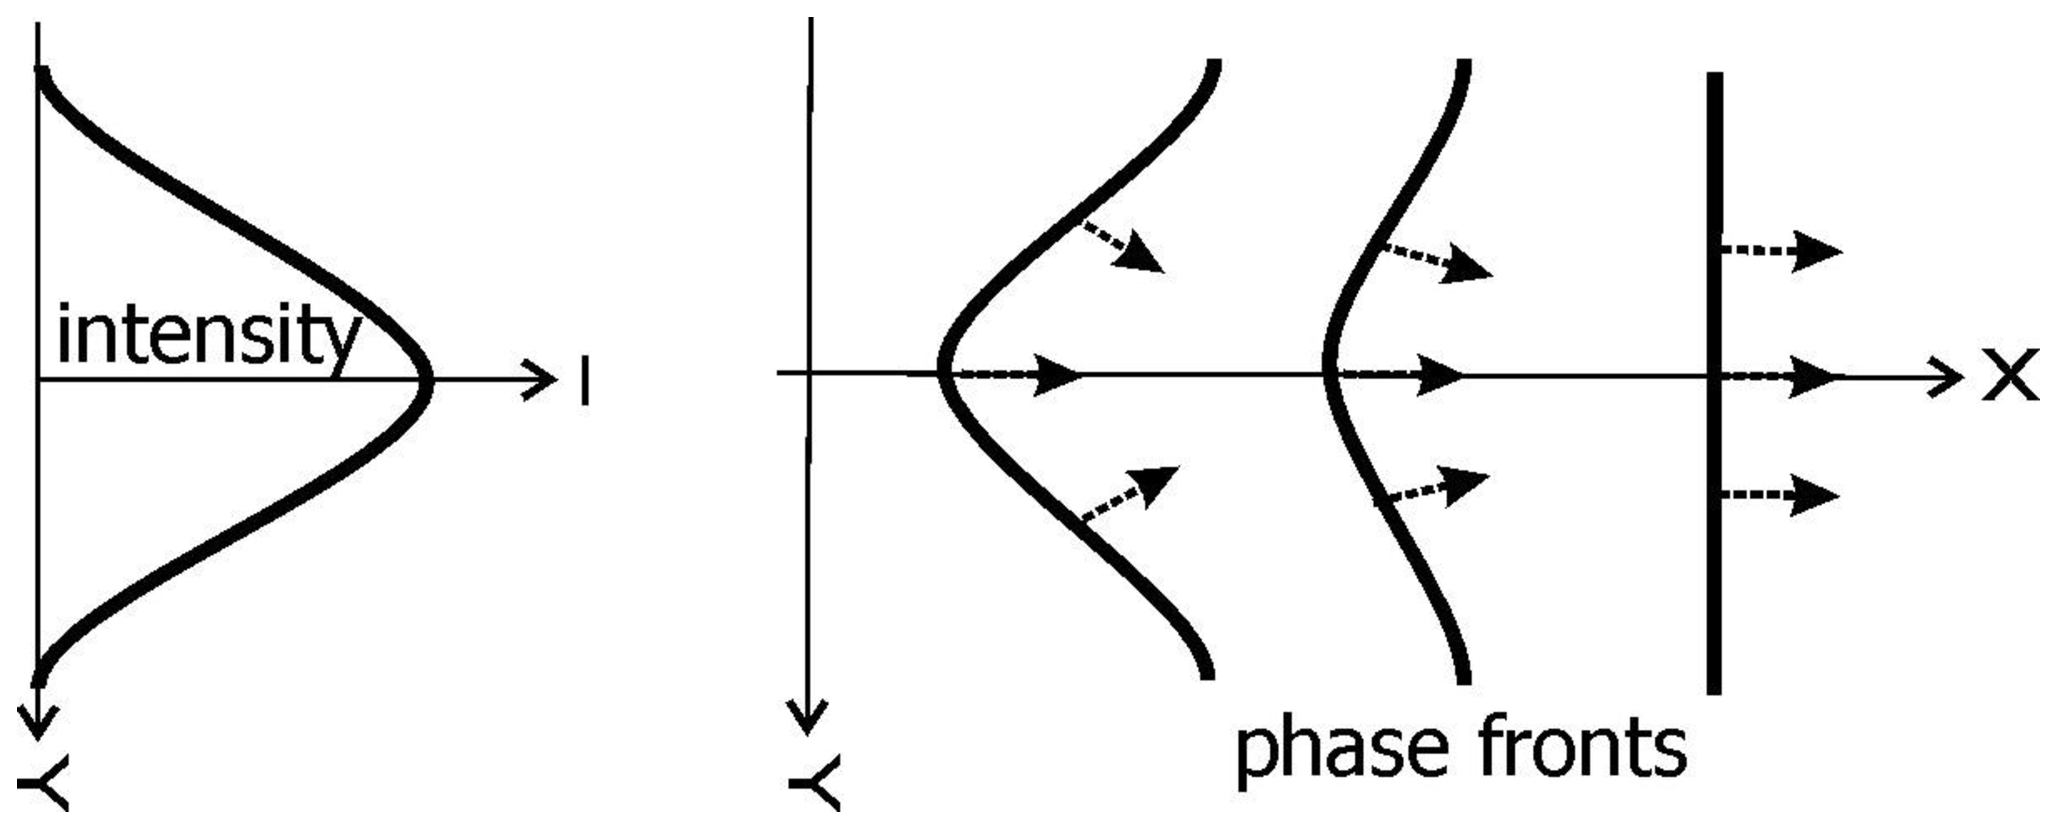
\includegraphics[width=\MyFactor\textwidth]{Img/selffocussing.eps}
  \caption{激光自聚焦示意图}
  \label{fig:selffousing}
\end{figure}

\begin{figure}[!htbp]
  \centering
  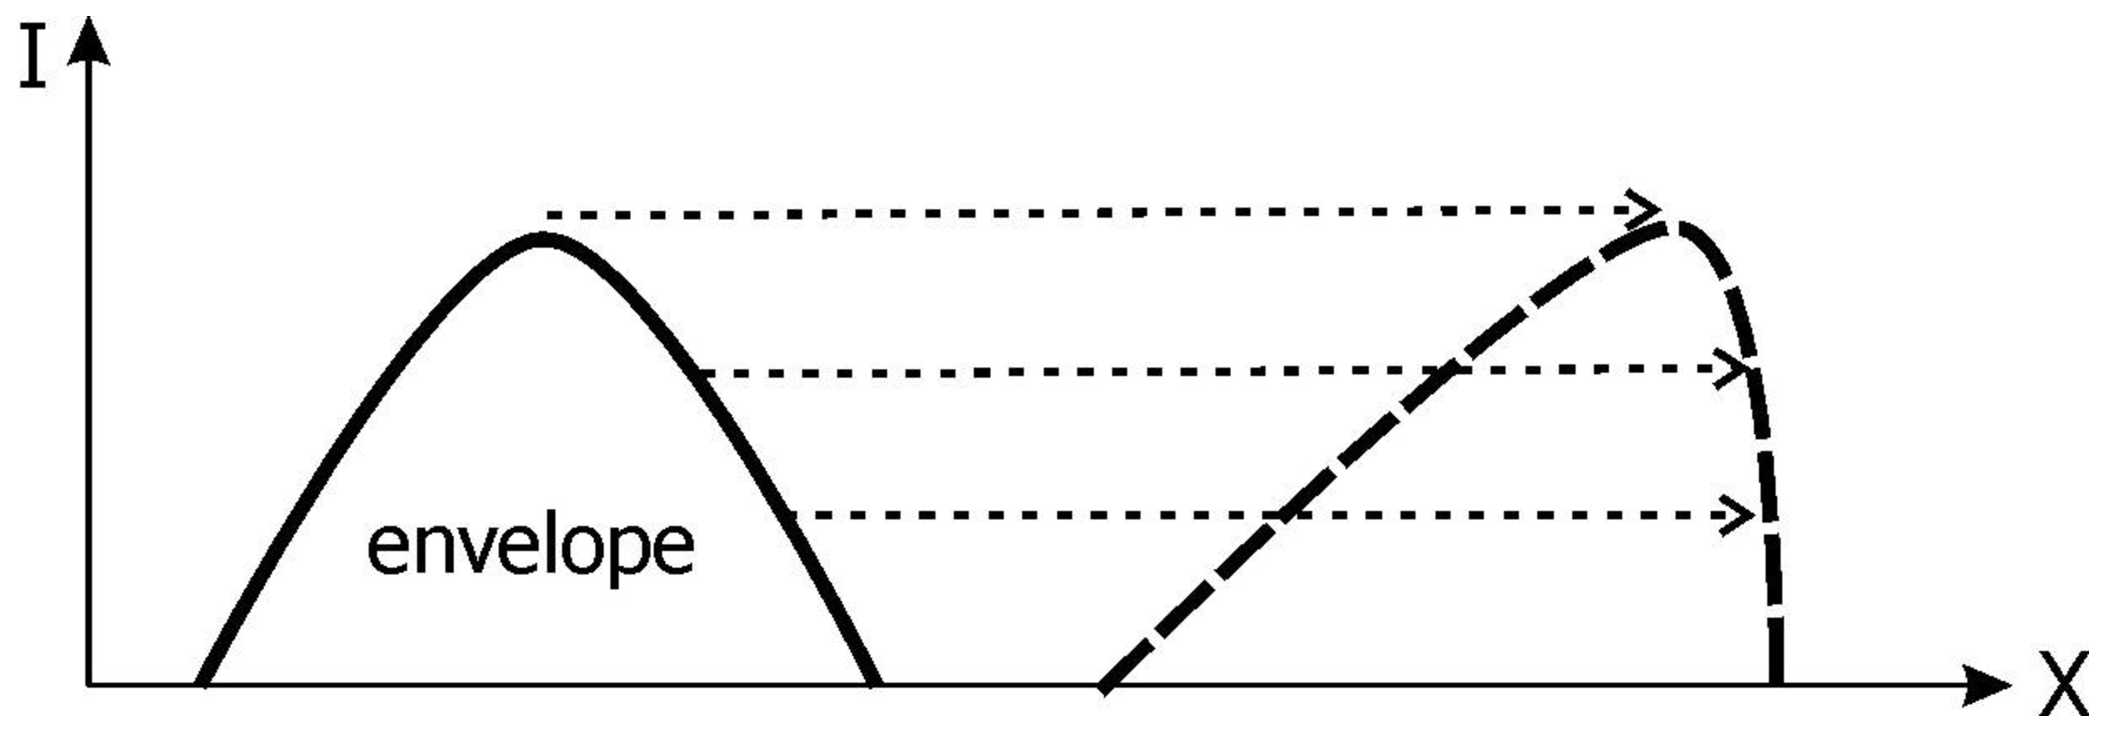
\includegraphics[width=\MyFactor\textwidth]{Img/prof-steepening.eps}
  \caption{激光自相位调制}
  \label{fig:phaseModulate}
\end{figure}




在激光在等离子体传播的过程中,存在很多的非线性机制。由于激光脉冲横纵向分布,对于等离子体折射率的调制,会产生相对论自聚焦以及相对论相位自调制现象。相对论自聚焦,是由于纵向高斯分布激光使得折射率中间低两翼高,像棱镜般对于激光脉冲形成聚焦效果,横向尺寸变小。另一方面,纵向高斯分布使得激光波前群速度较低,发生相对论相位自调制,使得激光脉冲纵向压缩。最终,由于相对论自聚焦以及自调制作用,激光的峰值光强得到明显的提高,横纵向尺寸得到有效的压缩\cite{wang2011laser}。
与此同时,激光脉冲前沿的电子被激光有质动力排开,形成横向尺寸与激光焦斑大小相当的离子通道结构。通道中电子密度中间低,通道壁较高,且一部分电子在通道壁回流产生磁场。然而离子分布均匀,电子与离子在通道中静电分离,通道中形成了的静电势,通道中的电子  在静电势中作betatron震荡。此外,这些betatron共振电子受到激光场的驱动作用,当betatron震荡频率与激光频率匹配时,共振现象发生,使得电子产生强烈的能量吸收,这种现象被称为DLA(Direct Laser Acceleration)。共振电子的横向震荡频率即激光频率$\omega_0$,纵向的频率由于  是$2 \omega_0$。共振电子产生之后沿激光方法传播,同时由于通道壁电子回流产生的磁场聚焦作用,形成高能量密度的束流。关于DLA的系统研究属于A. Pukhov和J. Meyer-ter-Vehn以及盛正明\cite{pukhov1998relativistic,pukhov1999particle},通过模拟和实验,得出电子的温度的定标率,
\begin{equation}
\label{eqn:DLAtemperature}
T_e = 1.8(I_{cpa} {\lambda}^2/{13.7}GW)^{1/2}
\end{equation} 

相对于同等光强的相对论有质动力加热,其温度有三倍以上的提高,且电子的能量密度较高,于是将共振电子用于质子加速能够有效。

\begin{figure}[!htbp]
  \centering
  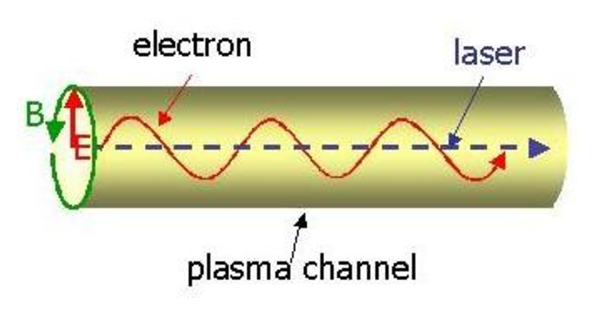
\includegraphics[width=\MyFactor\textwidth]{Img/IFEL.eps}
  \caption{逆自由电子激光示意图}
  \label{fig:IFEL}
\end{figure}


在我们的加速方案中,使用激光预脉冲产生预等离子体,激光主脉冲与预脉冲作用产生DLA共振电子。激光能量有效地转化给电子,而后电子传播至靶后形成鞘层场加速离子,最终对于离子加速产生增强的作用。整个加速方案的模型,首先强度$10^{12}W/cm^2$,脉冲时间$100ps$量级烧蚀脉冲与$\mu m$量级的金属靶作用。通过调整烧蚀脉冲的强度以及持续时间,控制金属靶的烧蚀深度和预等离子体膨胀距离以及密度梯度,最终得到指数密度分布预等离子体与未烧蚀金属靶的双层靶结构。而后相对论强度的激光与双层靶作用,首先激光脉冲在预等离子体临界密度区域中产生高能量高密度的DLA共振加热电子,共振电子传输到靶后面,在靶后建立起鞘层静电加速场。未烧蚀的金属靶的作用,提供质子层并提供未破坏的后表面。在这一模型的基础上,我们对于加速有如下的理论估计:
首先,加速的过程是在后表面由于电子产生的鞘层加速场产生的,仍然归类为TNSA加速机制。
相对于有质动力加热,其电子温度大约三倍,且其能量密度较高。
对于加速时间,我们采用fuchs的 $1.3 t_{laser}$的估计。 利用TNSA理论中,估计质子的能量增加至少三倍,而电子的温度是重要原因。


问题的关键在于如何确保电子的温度可以达到最大值,而且保证高能量高密度的电子可以传播达到靶的后面。DLA电子高能高密,是由于共振效应,以及通道中磁场的聚焦效果的作用。因此电子能量密度,重要的条件是通道的存在,使得电子达到固体靶之前(因为固体靶中的电子由于相互之间的空间电荷力产生的密度减小可以忽略)仍然保持高度的聚焦状态。因此最优的加速条件:
激光在即将达到固体靶的时候耗尽所有的能量,即DLA共振电子获得最大程度的能量增益的同时,确保激光脉冲产生的通道能够一直连接到金属靶,有助于电子保持聚焦的高密度状态。
电子的加热和传输在很大程度上决定于等离子体的密度,而预等离子体的分布由预脉冲决定,因此可以通过控制预脉冲的参数,满足最优条件。对此我们有如下的估计: 1 通道横向尺寸与激光相当;




